\chapter{Применение предложенных подходов}

В этой главе приводится описание применения предлагаемой в диссертации технологии 
для разработки различных предметно-ориентированных решений. В силу ограниченности 
объёма диссертации были выбраны три наиболее зрелых решения: QReal:Robots, QReal:Ubiq,
QReal:Hascol. Все эти решения имеют достаточно сильно различающиеся предметные области 
и разнятся по применённым в них подходам к созданию предметно-ориентированных языков. 
Соответственно, результирующие предметно-ориентированные языки достаточно сильно отличаются 
друг от друга, что является аргументом в пользу широкой применимости предлагаемой технологии.

	В этой главе приводится описание применения предлагаемой в диссертации технологии для разработки различных предметно-ориентированных решений. В силу ограниченности объёма диссертации были выбраны три наиболее зрелых решения: QReal:Robots, QReal:Ubiq, QReal:Hascol. Все эти решения имеют достаточно сильно различающиеся предметные области и разнятся по применённым в них подходам к созданию предметно-ориентированных языков. Соответственно, результирующие предметно-ориентированные языки достаточно сильно отличаются друг от друга, что является аргументом в пользу широкой применимости предлагаемой технологии.
5.1. Среда программирования роботов QReal:Robots
	Наиболее зрелый на данный момент пример применения технологии QReal - среда для обучения программированию в школах QReal:Robots. Этот проект создавался в практически идеальных для применения предметно-ориентированного подхода условиях: имелась достаточно узкая предметная область, в которой уже довольно активно применялось визуальное программирование, имелась потребность в средствах программирования в рамках этой предметной области для написания нетривиальных программ, имелась DSM-платформа QReal, на которой было возможно в короткие сроки реализовать такое решение. В этой работе результаты проекта QReal:Robots изложены достаточно кратко, более подробно см. статьи [ссылка на статьи про QReal:Robots, коих к моменту окончания работы над текстом будет минимум 4]. Далее описание результатов приводится в такой последовательности - приводится введение в предметную область и мотивация к созданию DSM-решения, анализ и формулировка требований, изложение возможностей визуального языка и инструментальных средств для него с точки зрения пользователя и “ручной” реализации, далее рассказывается, как при реализации DSM-решения применялись возможности платформы QReal, в чём она смогла помочь, а в чём нет, и почему.
5.1.1. Постановка задачи
	Сейчас в школах для начального преподавания информатики активно внедряются робототехнические конструкторы, наиболее популярный из которых на данный момент - конструктор LEGO Mindstorms NXT 2.0. Идея использовать роботы для преподавания не случайна, понятие "исполнитель" традиционно используется в школьном преподавании в России со времён академика Ершова, а робот - наиболее наглядный вид исполнителя. Исполнитель - это некая сущность, способная выполнять команды, указанные в программе, в некоторой среде. До сих пор самым популярным исполнителем в школах остаётся "черепашка" LOGO[ссылка], предложенная американским педагогом Сеймуром Пейпертом ещё в 1967 году. “Черепашка” может перемещаться по экрану, оставляя за собой след, и подчиняется командам вида “поднять перо”, “опустить перо”, “20 шагов вперёд”, “на 90 градусов налево”. В текстовых программах может быть неочевидно, где исполнение алгоритма пошло не так, а иногда непонятно даже, правильно работает программа или нет. В случае с “черепашкой” отклонение выполнения программы от задумки автора будет видимо сразу же, “черепашка” нарисует что-то некорректное. При этом сразу видно, где допущена ошибка, можно легко найти строку программы, на которой “черепашка” отклонилась от задуманной траектории.
	Исполнитель, движущийся по экрану, всё же оказывается недостаточно нагляден. Сеймур Пейперт в своих ранних экспериментах использовал механическую черепашку. Сейчас развитие электроники сделало возможным создавать относительно недорогие устройства, исполняющие программу с помощью дистанционного управления с компьютера или позволяющие загружать программу для автономного исполнения. Для преподавания в школах из таких устройств наиболее интересны робототехнические конструкторы, потому что они требут сборки робота перед его программированием, что интереснее для детей и развивает их конструкторские навыки. Самый известный такой конструктор - Mindstorms NXT. Он позволяет из трёх моторов, трёх видов датчиков (датчика касания, ультразвукового датчика расстояния, датчика освещённости), блока управления и пластмассовых деталей собирать довольно сложные конструкции, от движущихся тележек до стационарных устройств, например, для росписи ёлочных украшений или игры на барабанах. 
	Программировать такие роботы сложнее, чем “черепашку”, поскольку из конструктора можно собрать самые разные модели роботов, и программировать приходится в терминах, например, вида “мотор А включить на 50% мощности”, “ждать срабатывания датчика касания”, а не “вперёд на 20 шагов”, как в “черепашке”. Это интереснее и полезнее для детей, но сложнее. Дополнительную сложность добавляет и то, что робот может взаимодействовать с окружением с помощью датчиков, в отличие от “черепашки”. Это позволяет преподавать не только основы информатики, но и основы кибернетики, демонстрируя принципы построения программ, работающих во внешней среде, которую они не могут контролировать. Типичный пример задачи, которую решают начинающие программисты с помощью робота - движение по линии, когда робот с одним или двумя датчиками освещённости должен проехать по чёрной линии, нарисованной на полу. На “черепашке” обучать решению подобных задач невозможно.
	Сложность программирования робототехнических конструкторов преодолевается использованием визуальных языков программирования. Они гораздо понятнее и нагляднее для школьников, чем текстовые языки. Программы на таких языках состоят из элементарных блоков, например, “включить мотор”, “ждать срабатывания датчика”, которые достаточно перетащить с палитры на диаграмму и соединить связями. При наличии удобного редактора для такого языка пользоваться им могут даже дошкольники, не умеющие ещё читать. Как правило, с помощью визуальных языков школьники программируют примерно до седьмого класса, после чего постепенно переходят на текстовые языки. В комплекте с конструктором поставляется среда визуального программирования NXT-G[ссылка], существуют отдельно распространяемые среды, самой популярной из которых в школах является Robolab[ссылка]. Визуальное программирование в сообществе людей, занимающихся программированием таких роботов, весьма популярно.
	Существующие среды программирования роботов имеют ряд недостатков, затрудняющих их использование в школах, например, отсутствие русификации, невозможность отладки программы. Это делает актуальной задачу создания новой такой среды, учитывающей все достоинства и недостатки существующих, а также уже накопленный опыт преподавания. Поэтому возникла ситуация, чрезвычайно интересная для апробации DSM-платформы. В выбранной предметной области уже сложились традиции использования визуальных языков, поэтому можно рассчитывать на содержательное сравнение с существующими средами. Кроме того, задачи, решаемые в данной предметной области, достаточно нетривиальны, чобы полученный опыт разработки визуального языка можно было перенести на более сложные случаи, возникающие при промышленно программировании. Все типичные для императивного программирования конструкции, такие как ветвления и циклы, используются при программировании роботов, поэтому полученные результаты окажутся применимыми и для других случаев, где требуется императивный подход.. Вместе с тем, предметная область достаточно узка, чтобы можно было получить заметные выгоды от использования предметно-ориентированного языка: на языке общего назначения программирование велось бы путём вызова функций API робота, для чего требовалось бы писать довольно много вспомогательного кода, например, объявления функций. Кроме того, при использовании визуального языка невозможно совершить некоторые ошибки, типичные для текстовых языков, например, невозможно ошибиться в написании имени вызываемой функции, если достаточно просто перетащить соответствующий ей блок из палитры.
5.1.2. Существующие среды визуального программирования роботов
Как уже отмечалось, визуальное программирование весьма популярно среди людей, работающих с конструкторами Mindstorms. Анализ существующих сред является естественным источником для формулировки требований к проектируемому DSM-решению, наряду с интервьюированием экспертов в предметной области и потенциальных пользователей. Результаты анализа существующих сред представлены ниже.
Среда NXT-G[ссылка] поставляется вместе с конструктором Mindstorms NXT. Среда базируется на системе визуального программирования LabView[ссылка], используемой для моделирования различных экспериментов. Среда LabView в качестве языка программирования использует визуальный язык G, язык с процессом вычислений, ориентированным на данные - в нём связи между блоками обозначают не последовательность выполнения операторов, а зависимости между блоками по данным. Основная проблема среды NXT-G заключается в отсутствии полноценной поддержки математических выражений. В языке присутствуют блоки для арифметических действий, констант, переменных, и чтобы построить математическое выражение, их надо соединять связями. Таким образом, на диаграмме приходится рисовать фактически дерево разбора арифметического выражения, что делает программирование даже несложных задач, требующих математики, чрезвычайно утомительным. В школьной программе такие задачи возникают часто, например, движение по линии или езда вдоль стены с помощью датчика расстояния требует вычисления производной, поэтому NXT-G для преподавания в школах практически не используется. Ещё одной особенностью этой среды, оказавшейся недостатком при преподавании в школах, стало то, что не все свойства блоков видны на диаграмме, требуется кликнуть на блок и открыть его свойства в редакторе свойств. Это делает невозможным показ всей программы на проекторе, что затрудняет воспроизведение программы учениками. У NXT-G нет официальной русификации, отсутствуют встроенные средства отладки и генерации текстовой формы языка. Возможно добавление сторонних блоков средствами LabView, сам NXT-G позволяет выделять фрагменты диаграмм в подпрограммы и использовать их с помощью специального блока.
Среда Robolab[ссылка] также создавалась на основе среды LabView, и, в отличие от NXT-G, создавалась специально для преподавания. Примером специфичного для преподавания решения, принятого в среде Robolab, может послужить разделение возможностей среды на уровни. При запуске среды предлагается выбрать уровень, на котором будет вестись работа, на первых уровнях пользователь может только заполнять пустые места в уже готовом шаблоне программы, используя очень ограниченный набор блоков. На более высоких уровнях предоставляется возможность самостоятельно задавать связи между блоками, доступно больше различных видов блоков (например, на начальном уровне есть блок “ждать”, на более высоком - набор блоков “ждать 1 сек”, “ждать 2 сек”, “ждать 5 сек” и т.д., на ещё более высоком - “ждать N сек”, где N является параметром блока и может являться результатом вычисления. Такое разделение позволяет начать работу со средой детям дошкольного возраста, которые не умеют ещё даже читать (картинки, используемые в блоках, достаточно понятны), при этом дети могут исследовать среду и разбираться в функциональности более высоких уровней постепенно, практически без помощи преподавателей.
Математические выражения Robolab поддерживает гораздо лучше, чем NXT-G, позволяя писать произвольные выражения в виде текста, используя тригонометрические функции и переменные, обращаться к значениям, возвращаемым датчиками, прямо из выражений. Циклы в Robolab реализованы довольно необычно - есть блоки “начало цикла” и “конец цикла”, связь между концом и началом никак не визуализируется. Есть довольно развитая поддержка параллельных задач, есть все необходимые конструкции императивного программирования, включая подпрограммы. Русифицирована среда лишь частично, не имеет встроенных средств отладки, не может порождать код программы в текстовом виде, имеет довольно несовременный пользовательский интерфейс, при этом небесплатна и стоит довольно дорого для российских школ. При этом, несмотря на все перечисленные недостатки, эта среда вполне подходит для иллюстрации материала информатики и кибернетики примерно до 7-го класса школы, и сейчас является самой распространённой в школах России.
Среда Microsoft Robotics Developer Studio (MRDS), в отличие от рассмотренных ранее сред, не создавалась исключительно для конструктора Mindstorms NXT. Среда предназначена для создания сложных многопоточных приложений с реактивной моделью поведения, которые весьма типичны для задач робототехники - современная робототехническая система представляет собой целый комплекс вычислительных средств, часть из которых может быть установлена на роботе, а часть - на компьютере, связанном с роботом скоростной сетью. Кроме того, необходимость в высокопроизводительных распределённых программных системах возникает не только в робототехнике, поэтому среда MRDS применяется и в других областях, например, с её помощью разрабатывались серверные части крупных веб-приложений [ссылка на CCR at MySpace]. Программа в MRDS представляется в виде набора веб-сервисов, исполняемых независимо и обменивающихся данными друг с другом. Процесс программирования сводится к связыванию входов и выходов предопределённых сервисов, что осуществляется на визуальном языке VPL (Visual Programming Language). Этот язык, таким образом, попадает в категорию языков с процессом управления, ориентированным на данные, чем очень похож на визуальные языки систем, рассмотренных выше. Среда имеет развитую трехмерную среду симуляции, позволяя исполнять созданные программы не только на реальном роботе, но и на трёхмерной модели в окружении с подробной симуляцией физики (например, в стандартной поставке имеется подробная трёхмерная модель квартиры, по которой может перемещаться робот). Среда поддерживает генерацию кода на языке C#, отладку, распространяется бесплатно.
Несмотря на всё это, среда MRDS очень редко используется в школах для преподавания информатики. Связано это прежде всего с используемой там моделью вычислений. Представлять программу в виде взаимодействующих независимо исполняющихся веб-сервисов удобно профессиональным программистам, но школьникам, впервые пробующим программировать, потребуется знать и уметь слишком многое, чтобы писать содержательные программы. К тому же, такой подход к программированию слишком специфичен и не может быть использован в качестве иллюстративного материала для “обычного” императивного программирования, знание которого будет необходимо школьникам в дальнейшем. Кроме того, генерируемый средой код не может быть исполнен непосредственно на роботе Mindstorms NXT - он имеет слишком мало ресурсов для этого, робот может управляться только дистанционно по интерфейсу Bluetooth. Среда MRDS ориентирована на более дорогие устройства, в частности, “стандартная модель” робота, рекомендуемая для использования в MRDS включает в себя ноутбук в качестве блока управления, который один дороже всего конструктора Mindstorms NXT. Использование модели робота позволяет решить эту проблему только частично - модель, даже с детальной реализацией физических эффектов, не позволяет воспроизвести всё многообразие реального мира, из-за которого, собственно, и возникают проблемы, которые решаются в кибернетике.
5.1.3. Требования к DSM-решению
	По результатам анализа существующих сред и общения с экспертами предметной области (преподавателями и методистами, использующими робототехнические конструкторы в своей работе) были сформированы следующие требования к проектируемому DSM-решению.
Среда должна позволять создавать довольно сложные программы, поскольку предполагается, что она будет служить для иллюстрации нетривиальных вопросов информатики и кибернетики, при этом её язык должен оставаться близким к “традиционным” императивным языкам программирования. Среда должна удобно поддерживать нетривиальные математические выражения, переменные, ветвления, циклы, параллельные задачи.
Среда должна быть проста и удобна в работе, поскольку неудобный пользовательский интерфейс создавал бы дополнительную когнитивную нагрузку при изучении и без того сложного материала. Среда должна быть интуитивно понятна, работа со средой должна быть возможна при минимальном участии преподавателя.
Требуется наличие встроенных средств отладки, поскольку школьникам важно не столько сделать работающую программу, сколько разобраться в том, как она работает. Ошибки могут иметь большую педагогическую ценность, и среда должна иметь возможность демонстрировать ошибки (и ход выполнения программы вообще) школьникам. Весьма желательна возможность исполнения программы на модели робота на компьютере
Требуется наличие возможности порождения текстового представления программы. Школьники старших классов, серьёзно занимающиеся программированием, должны видеть связь между диаграммами и кодом на текстовых языках, иметь возможность редактировать текстовую программу в той же среде, в которой они привыкли работать.
Среда должна быть русскоязычной, поскольку основная группа её пользователей ещё не владеет в должной степени иностранными языками.
	Как видно из приведённого выше обзора, ни одна из существующих сред программирования роботов указанным требованиям не удовлетворяет. Наиболее активно в школах используется среда Robolab, но, поскольку он недёшев, среди школьных учителей есть желание заменить её на более современный (и по возможности бесплатный) аналог. Поэтому существует реальная потребность в создании новой такой среды, что и было сделано на базе метатехнологии QReal.
5.1.4. Визуальный язык QReal:Robots
	В качестве модели вычислений для визуального языка в силу наличия требования близости к “традиционным” языкам программирования была выбрана модель вычислений, ориентированная на поток исполнения. Блок языка представляет собой элементарную команду роботу, связи между блоками указывают последовательность, в которой выполняются блоки, это делает программы больше похожими на блок-схемы, чем программы на существующих средах программирования роботов. Пример программы приведён на рисунке [номер рисунка]. Двухмоторная тележка с датчиком касания под управлением этой программы будет двигаться до срабатывания датчика касания, после чего подаст звуковой сигнал и будет некоторое время двигаться в обратном направлении, после чего повторит действия сначала.
Рисунок [номер рисунка]. Пример программы QReal:Robots.

	Все блоки языка разбиты на смысловые группы, которые могут быть отдельно свёрнуты или развёрнуты в палитре. Описание для каждого блока приведено ниже.
Группа “Алгоритмы” предназначена для блоков, определяющих последовательность выполнения команд программы.
“Диаграмма поведения робота” - блок, на который добавляются все остальные блоки программы. Обычно непосредственно в рабочей области не рисуется, но при создании новой диаграммы перетаскивается из палитры в обозреватель модели.
“Линия соединения” - единственная связь, присутствующая в языке, задаёт последовательность исполнения блоков. Имеет метку, которая позволяет определять, когда управление надо передать по линии соединения в случае условного оператора или цикла - например, метка “больше 0” говорит, что управление по данной связи будет передано только тогда, когда выражение в условном операторе, подключённом к этой связи, будет иметь значение, большее 0. По умолчанию связи не помечены ничем.
“Условие” - условный оператор. Параметризуется арифметическим выражением и должен иметь две исходящие связи, одна из которых выбирается для передачи управления в зависимости от значения выражения и метки связи.
“Цикл” - оператор цикла, параметризуется арифметическим выражением, значение которого будет количеством итераций, которые надо выполнить, и должен иметь две исходящие связи. Пока блок посещён меньшее количество раз, чем желаемое количество итераций, управление передаётся по связи, помеченной как “итерация”, как только желаемое количество итераций достигнуто, счётчик сбрасывается, и управление передаётся по непомеченной связи.
Группа “Действия” содержит блоки, реализующие элементарные команды роботу.
“Гудок” - проигрывает звук фиксированной частоты и фиксированной длительности с заданной громкостью.
“Играть звук” аналогичен блоку “Гудок”, но позволяет настраивать частоту и длительность звука.
“Моторы вперёд” - включает моторы по заданным портам с заданной мощностью (в процентах от максимальной).
“Моторы назад” - аналогичен блоку “Моторы вперёд”, но включает моторы в противоположном направлении.
“Моторы стоп”  - отключить моторы на заданных портах.
“Параллельные задачи” - разветвляет исполнение программы на два или более параллельно исполняемых потока.
“Функция” - позволяет вычислить произвольное выражение, записанное в текстовой форме как параметр блока. Выражения в QReal:Robots могут использоваться везде, где могут использоваться числовые значения, блок “Функция” введён для удобства как выделенное место для вычислений.
Группа “Инициализация” содержит блоки, обозначающие начало и конец программы, и позволяющие задать начальное состояние различных подсистем робота.
“Блок инициализации” обозначает место, с которого начинается исполнение программы, и позволяет задать, какие датчики подключены к портам управляющего блока робота.
“Конец” - завершает работу программы и отключает моторы и датчики робота.
“Начало” - аналогичен блоку инициализации, но не позволяет задать конфигурацию датчиков. В случае его использования конфигурация датчиков берётся из настроек, либо вычисляется по использованию блоков работы с датчиками в программе. Используется в программах, не использующих датчики, либо использующих один-два датчика, не требующих сложного конфигурирования.
“Сбросить показания энкодера” - обнуляет показания датчиков оборотов моторов по выбранным портам.
Группа “Ожидания” содержит блоки, останавливающие выполнение программы (или одного из параллельных потоков) до наступления некоторого события.
“Ждать интенсивность цвета” продолжает выполнение, когда датчик цвета по данному порту вернёт требуемое значение.
“Ждать свет” аналогичен блоку “Ждать интенсивность цвета”, но работает с датчиком света. Поясним, что набор Mindstorms NXT распространяется с датчиком цвета, который способен различать шесть цветов (красный, зелёный, синий, жёлтый, чёрный, белый), и измерять интенсивность света в одном из трёх режимов подсветки (красным, зелёным или синим цветом), или без подсветки (в пассивном режиме). Кроме этого, набор может использовать датчик света, распространявшийся в более разних версиях конструктора. Этот датчик может только измерять интенсивность света с красной подсветкой или без подсветки, распознавать цвета не может. Кроме того, есть ещё датчик цвета стороннего производителя, аналогичный по характеристикам датчику цвета из Mindstorms NXT, но способный распознавать больше цветов, QReal:Robots его на данным момент не поддерживает.
“Ждать сенсор касания” продолжает выполнение, когда срабатывает датчик касания.
“Ждать сонар” продолжает выполнение, когда ультразвуковой датчик расстояния возвращает значение в требуемых границах. 
“Ждать цвет” продолжает выполнение, когда сенсор цвета возвращает заданный цвет. Заметим, что в режиме распознавания цвета датчик цвета не может измерять интенсивность, поэтому данный блок не может быть использован вместе с блоком “Ждать интенсивность цвета” для датчика на том же порту.
“Ждать энкодер” продолжает выполнение, когда датчик оборотов мотора на заданном порту вернёт заданное значение.
“Таймер” продолжает выполнение программы по истечении заданного временного интервала (в миллисекундах).
Группа “Сегвей” содержит блоки, предназначенные специально для балансировки робота-сегвея с использованием средств операционной системы nxtOSEK и библиотеки NXTway-GS. Они были добавлены в палитру как демонстрация возможностей по использованию специфических функций операционной системы и сторонних библиотек, написанных на текстовых языках, а также как зрелищная демонстрация возможностей среды (балансирующий на двух колёсах робот привлекал внимание даже серьёзно увлекающихся робототехникой школьников, многие из которых затем интересовались средой, в которой он был запрограммирован).
"Балансировка" - вызов функции balance_control библиотеки NXTway-GS. Блок принимает текущие показания датчиков оборотов моторов и другие параметры, связаные с текущим положением робота, получает данные с гироскопа, и записывает в переданные переменные мощности моторов, которые надо выставить, чтобы робот сохранял вертикальное положение.
"Инициализация балансировки" - блок, вызывающий функцию balance_init библиотеки NXTway-GS. Она должна вызываться в начале работы программы, когда сегвей зафиксирован в вертикальном положении, и инициализирует внутренние переменные программы балансировки, в частности, показания гироскопа в вертикальном положении.
	Язык позволяет везде, где могут быть использованы численные значения, использовать и математические выражения. Выражения могут состоять из чисел, арифметических операций, переменных, специальных переменных, содержащих текущие значения сенсоров (называемых сенсорными переменными), тригонометрических функций. Все выражения (и все переменные) всегда имеют вещественный тип, переменные не объявляются, а начинают существовать в месте первого использования. Зависимости между блоками по данным никак не визуализируются, если один блок использует переменную, которой присваивается значение в другом блоке, то корректная последовательность исполнения этих блоков - ответственность программиста. 
	Пример программы, использующей математические вражения, приведён на рисунке [номер рисунка]. Эта программа решает задачу движения робота по чёрной линии, нарисованной на полу - самую популярную задачу на различных соревнованиях по робототехнике. Приведённое решение использует робот с двумя датчиками цвета и двумя моторами, независимо приводящими в движение колёса по бокам робота. Вычисляется разность между показаниями сенсоров, которые должны находиться по разные стороны от линии. Если, например, левый сенсор видит белую область, а правый - чёрную, робот сьезжает с линии влево, и ему надо довернуть вправо, чтобы остаться на линии. Умноженная на некий подбираемый эмпирически коэффициент эта разность становится управляющим воздействием на моторы, которое прибавляется к мощности одного мотора и вычитается из мощности другого, тем самым обеспечивая доворот робота.
Рисунок [номер рисунка]. Движение по линии.
	Интуитивная понятность программы обеспечивается приёмом, часто используемым при проектировании предметно-ориентированных языков: для изображения блоков используются иконки с изображениями, понятными людям, видевшим робот. На блоках управления моторами нарисованы моторы Mindstorms NXT, блоки работы с датчиками выполнены более абстрактно, но тоже интуитивно понятны. Это позволяет успешно пользоваться средой даже людям, которые впервые её видят, но знакомы с конструктором. Кроме того, оказалось важно, что связи рисуются со стрелками на концах, в других средах связи стрелок не имели, и пользователи обратили на это внимание - со стрелками им показалось гораздо понятнее. Это оказалось довольно неожиданным, поскольку направления связей всегда очевидны, и стрелки создавались исключительно как декоративные элементы - для пользователей предметно-ориентированного языка может оказаться важным то, что кажется совершенно неважным авторам языка.
5.1.5. Инструментальные средства QReal:Robots
	С помощью технологии QReal оказалось легко создать визуальный язык и редактор для него, однако инструментальные средства, такие как симулятор робота (далее называемый “двухмерная модель”), интерпретатор диаграмм, управляющий роботом удалённо, генератор кода для загрузки на робота пришлось создавать вручную. Ниже представлен краткий обзор созданных вручную инструментальных средств.
	Наиболее объёмным по коду и сложным в реализации является интерпретатор диаграмм. Интерпретатор принимает на вход репозиторий с диаграммой поведения робота, и исполняет её, в зависимости от режима, либо на настоящем роботе посылкой ему команд по интерфейсу Bluetooth или USB, либо на двухмерной модели робота. Интерпретатор создавался с учётом следующих требований.
Возможность исполнять программу, управляя роботом по Bluetooth или USB, в зависимости от выбора пользователя.
Возможность исполнять программу на двухмерной модели робота. Двухмерная модель должна эмулировать окружение, способное взаимодействовать со всеми видами сенсоров - должна быть возможность задать положение стен, фиксируемых датчиками касания и расстояния, и непроходимых для робота, и разноцветных линий на полу, видимых для датчиков света и цвета.
Архитектура интерпретатора должна позволять быстро (в течение единиц часов) добавлять поддержку новых блоков визуального языка, и новых видов оборудования. Должна быть возможность относительно просто и без серьёзных изменений в архитектуре поддержать новые виды устройств, включая другие робототехнические конструкторы, отличные от NXT, но имеющие схожую архитектуру.
	Архитектура интерпретатора представлена на рисунке [номер рисунка]. 
Рисунок [номер рисунка]. Архитектура интерпретатора.
	Главный класс, который предоставляет свои функции графическому интерфейсу пользователя и может быть вызван из ядра системы - Interpreter. Он содержит в себе логическую модель робота, таблицу блоков и список активных потоков. Логическая модель робота (класс RobotModel) играет роль программного интерфейса к устройству, и состоит из объектов (наследников RobotPart), каждый из которых реализует программный интерфейс к какому-либо элементу робота - одному из датчиков, мотору, блоку управления. Эти объекты предоставляют высокоуровневые команды, которыми можно пользоваться при реализации поведения блока визуального языка, например, включение мотора, проигрывание звука. Таблица блоков - это отображение блоков на диаграмме на объекты, реализующие их поведение. Для каждого блока языка существует свой класс (наследник Block), который его реализует, способный принять управление, выполнить какое-то действие (возможно, асинхронно), и вернуть интерпретатору следующий блок, который надо выполнить. Объекты этих классов создаются для каждого блока при начале работы интерпретатора и помещаются в таблицу, чтобы, когда управление дойдёт до какого-либо блока на диаграмме, найти по идентификатору блока соответствующий ему объект в таблице.
	Логическая модель робота и её составные части могут быть реализованы по-разному, давая возможность прозрачно для реализации блоков исполнять программу на реальном роботе, двухмерной модели, или, потенциально, другом устройстве. Для реализации этого использован паттерн “Мост”, дающий возможность для иерархии классов, видимых реализациям блоков, использовать заменяемые реализации. Модель робота содержит ссылку на реализацию модели робота, которая может быть либо логической моделью реального робота, либо логической моделью двухмерной модели, либо пустой моделью (модель, которая не посылает команды никуда, а просто эмулирует некоторое фиксированное поведение, полезна для начальной отладки программы). Каждый класс, представляющий датчик, имеет ссылку на реализацию, которая тоже может быть одного из трёх видов, аналогично самой модели. Конкретная модель может создавать модели датчиков своего типа, поэтому достаточно инициализировать интерпретатор требуемым типом модели, вся дальнейшая необходимая инициализация выполнится автоматически.
	В случае с двухмерной моделью классы-реализации элементов модели перенаправляют запросы в объект класса D2RobotModel. Этот класс занимается собственно симуляцией робота, обсчитывая его перемещение, реакции на команды от классов-реализаций. Внешнее окружение моделирует отдельный класс WorldModel, и D2RobotModel может запрашивать показания датчика в заданной позиции и с заданным направлением у этого класса. Отображением результатов симуляции занимается класс D2ModelWidget. Архитектура этой части системы представлена на рисунке [номер рисунка].
Рисунок [номер рисунка]. Архитектура двухмерной модели.
	Управление роботом по интерфейсам Bluetooth и USB использует одну логическую модель робота, класс RealRobotModel. Это оказалось возможно, потому что оба эти интерфейса используют одинаковый набор команд в примерно одинаковом формате, разнятся лишь заголовки пакетов с командами, передаваемых на робот. Поэтому оказалось возможным вынести транспортный уровень в отдельный набор классов, где инкапсулирована низкоуровневая работа с каналами передачи, и логическая модель просто параметризуется нужным транспортным уровнем. Транспорт для USB использует драйвер робота Fantom из поставки конструктора [ссылка], транспорт для Bluetooth работает непосредственно с системными средствами передачи (для работы с виртуальным COM-портом Bluetooth-канала используется сторонняя библиотека QextSerialPort[ссылка]). 
	Окно двухмерной модели представлено на рисунке [номер рисунка]. Двухмерная модель моделирует одну предопределённую конфигурацию робота - трёхколёсную тележку с двумя ведущими колёсами, используемую во многих задачах, связанных с движением (например, в робофутболе), однако можно задавать позицию и направление датчиков. Цветные линии на полу, видимые датчикам света и цвета, можно рисовать инструментами “Линия”, “Карандаш”, “Эллипс”, стены - инструментом “Стена”. Все элементы после размещения в рабочей области редактируемы, так что двухмерная модель близка по функциональности к простому векторному редактору. Имеется возможность сохранить нарисованную модель окружения в xml-файл.
Рисунок [номер рисунка]. Окно двухмерной модели.
	Генератор кода на текстовом языке реализован в виде отдельного подключаемого модуля и может работать независимо от интерпретатора. Он генерирует код на языке C с использованием программного интерфейса операционной системы nxtOSEK[ссылка], на данный момент считающейся самой быстрой операционной системой для роботов Mindstorms NXT. Для того, чтобы сгенерированный код можно было загружать на робот, требуется, чтобы на роботе была установлена nxtOSEK, а на компьтере с QReal:Robots - кросскомпилятор и комплект средств разработки для этой ОС. Всё необходимое для кросскомпиляции поставляется в виде отдельного инсталляционного пакета, который требует установленного QReal:Robots для установки. Решение не включать средства разработки в основной инсталляционный пакет QReal:Robots было принято из-за их большого объёма, что могло создать трудности при загрузке инсталляционного пакета пользователям, которым генерация текстовых программ не требуется. Генератор порождает .c-файл с кодом программы и .oil-файл с настройками её запуска, после чего запускается кросскомпилятор, собирающий бинарный образ программы, который потом загружается на робот по USB посредством утилиты из поставки конструктора. Для пользователя этот процесс прозрачен, ему достаточно нажать на кнопку “Загрузить” и дождаться сообщения об успешном завершении процесса загрузки. Если пользователю не требуется загружать программу на робот, он может просто сгенерировать код,  просмотреть и отредактировать его во встроенном в QReal:Robots текстовом редакторе с подсветкой синтаксиса.
	Генератор организован по шаблонной схеме: имеется файл с шаблоном порождаемого кода, в котором отмечены места, параметризуемые информацией из модели. Такие места, в свою очередь, могут сами заполняться текстами, сформированными с помощью шаблонов, и т.д., что позволяет генерировать сложно структурированные  повторяющиеся фрагменты кода. Пример шаблона верхнего уровня для генерации кода программы приведён ниже.

#include "kernel.h"
#include "ecrobot_interface.h"
@@BALANCER@@
@@VARIABLES@@

void ecrobot_device_initialize(void)
{
@@INITHOOKS@@
}

void ecrobot_device_terminate(void)
{
@@TERMINATEHOOKS@@
}

/* nxtOSEK hook to be invoked from an ISR in category 2 */
void user_1ms_isr_type2(void){ /* do nothing */ }

@@CODE@@

С помощью текста, заключённого в “@@”, отмечаются места для вставки параметризованного кода, так называемые заглушки (placeholders), генератор заменяет вхождения заглушек на сгенерированный для них по модели код. В приведённом выше примере заглушка @@BALANCER@@ заменяется на объявления функций и переменных для балансировки сегвея, если блоки работы с сегвеем используются на диаграмме, или пустой строкой, если таких блоков нет. @@VARIABLES@@ заменяется на объявления переменных - генератор в начале работы анализирует все арифметические выражения в программе, формирует таблицу переменных, и все объявления переменных генерирует на место этой заглушки. Заглушки @@INITHOOKS@@ и @@TERMINATEHOOKS@@ заменяются на код инициализации и деинициализации датчиков, зависящий от того, какие датчики использовались в программе. 
Заглушка @@CODE@@ заменяется на код, сгенерированный по диаграмме. По каждому блоку визуального языка генерируется свой небольшой фрагмент программы, реализующий поведение этого блока. Некоторую сложность представляют конструкции, управляющие потоком исполнения - условные операторы и операторы цикла. В отличие от структурных текстовых языков, где операторы образуют иерархическую структуру, визуальный язык позволяет связывать любой блок с любым блоком, что позволяет рисовать неструктурные программы, где поток управления попадает внутрь “тела” условного оператора или цикла извне. Это равносильно использованию оператора goto в текстовых языках, при этом визуальный язык QReal:Robots (как и многие другие подобные языки) не визуализирует структурные конструкции и нарушение структурности может произойти незаметно для программиста. Пример неструктурной программы приведён на рисунке [номер рисунка]. Генератор применяет ряд эвристик для анализа потока исполнения программы и поиска структурных условных операторов и циклов. В случае, если структурный код не может быть порождён по данной диаграмме (как, например, представленной на рисунке), генератор выдаёт ошибку и не генерирует код. Такое решение было принято всвязи со спецификой применения генератора - он должен порождать по возможности качественный и читаемый код, очевидным образом связанный с диаграммой, поскольку служит для обучения школьников программированию. Это исключает использование goto в сгенерированном коде, и делает нежелательным использование техник goto elimination[ссылка на оранжевую книжку про реинжиниринг], поскольку они предполагают раскопирование неструктурных участков кода. Интерпретация таких диаграмм, тем не менее, вполне возможна.
Рисунок [номер рисунка]. Пример неструктурной программы.
5.1.6. Опыт применения QReal
5.1.6.1. Метамодель языка QReal:Robots
	Визуальный язык QReal:Robots создавался в метаредакторе QReal. Метамодель одной из версий языка представлена на рисунке [номер рисунка]. Как видно, вся метамодель языка умещается на одном экране. Некоторая содержательная информация на рисунке не показана, поскольку она находится в свойствах элементов, и редактируется через редактор свойств (например, внешний вид элемента). Метмодель всё же слишком велика, чтобы на рисунке были видны все детали, поэтому ниже приводится словесное описание изображённого на рисунке.
Рисунок [номер рисунка]. Метамодель языка QReal:Robots.
	Корневым элементом любой диаграммы визуального языка является узел “Диаграмма” (сущность DiagramNode в метамодели). Она наследуется от узла “Диаграмма”, объявленного в импортированной метамодели KernelDiagram, получая от неё все свойства, там объявленные. Корнем иерархии наследования узлов языка является узел AbstractNode, который связан отношением Contains с DiagramNode, давая тем самым возможность всем своим наследникам располагаться на диаграмме. AbstractNode на рисунке [номер рисунка] имеется в двух экземплярах, поскольку от него наследуются все узлы языка, и отношения наследования, соединённые с одним AbstractNode, сделали бы диаграмму трудночитаемой - это пример применения принципа разделения логической и графической моделей. Для узла AbstractNode не задано графическое представление, поэтому он не будет отображаться в палитре, и не может быть использован на диаграммах. От AbstractNode наследуется несколько конкретных узлов, видимых в палитре, таких как InitialNode, FinalNode (блоки “Начало” и “Конец” соответственно), и два абстрактных узла - EngineCommand (блок управления двигателями) и SensorBlock (блок работы с датчиками). Эти узлы абстрактные, поскольку в них определяются свойства, общие для всех их потомков (например, порты, к которым применяются команды двигателей), сами они никакой смысловой нагрузки не несут и не видны в палитре. От EngineCommand наследуется абстактный блок EngineMovementCommand, имеющий свойство Power (мощность двигателя в процентах от максимальной), и конкретный блок EngineStop, который не требует параметра мощности, и поэтому не наследуется от EngineMovementCommand. Наследники EngineMovementCommand - блоки EnginesBackward и EnginesForward, которые никаких своих дополнительных свойств не имеют. Кроме блоков, в метамодели описано одно отношение (ControlFlow, “Поток управления”), и два типа-перечисления: SensorPort (порты, к которым может быть подключен датчик), и GuardType (тип условия над связью “Поток управления”, используемого в блоках “Условие” и “Цикл”).
5.1.6.2. Обсуждение
	Первые версии языка создавались в метаредакторе, первый прототип редактора был автоматически сгенерирован по метамодели в весьма короткие сроки - всего за два-три часа, из которых большая часть времени ушла на поиск иконок для отображения блоков. Возможность быстро получить редактор языка по метамодели и удобство редактирования метамодели в метаредакторе позволило не только существенно сократить время разработки языка, но и дать возможность экспериментировать, меняя свойства и внешний вид элементов. Кроме того, метамодель оказалось довольно удобно сопровождать, причём не только автору языка - работа над QReal:Robots в дальнейшем во многом была передана студентам, которые быстро разбирались в метаредакторе и могли самостоятельно добавлять в язык новые блоки или менять существующие. Рассматривалась даже возможность позволить самим пользователям менять свойства блоков языка (например, учителю скрыть ненужные в данный момент свойства блоков перед занятием), однако пока она не была востребована. Тем не менее, последние версии языка используют не графическую метамодель, а её XML-представление - за время работы над проектом XML-вариант метаязыка расширился новыми возможностями, которые не были реализованы в графическом метаязыке, например, задание групп блоков в палитре. Несмотря на это, вносить изменения в язык всё же достаточно просто для людей, занимавшихся разработкой QReal (например, студентов).
	Если технология сильно сократила время разработки визуального языка и редактора для него, то с созданием других средств инструментальной поддержки, таких как интерпретатора диаграмм или генератора кода, она смогла помочь в значительно меньшей степени. Это вполне ожидаемо, поскольку эти части содержат большое количество специфичных знаний предметной области, которые невозможно обобщить и вынести на метауровень, сделав частью технологии. Например, робот управляется удалённо так называемыми прямыми командами, которые можно посылать по интерфейсам Bluetooth или USB, и как формирование пакета с командой, так и логика работы с каналом передачи данных должны реализовываться вручную. Такого рода работы останутся трудоёмкими при любом уровне поддержки со стороны DSM-платформы, поскольку очень многое требуется изучить самому разработчику: систему прямых команд робота, API операционной системы робота для генерации кода в неё, работу с Bluetooth, USB, кросскомпиляцию, прошивку робота, загрузку программы на робот, и т.д. Тем не менее, DSM-платформа может взять на себя часть рутинной работы, и, предоставляя некий набор шаблонов и методологию, организовать и направить деятельность автора DSM-решения.
	Наиболее интересной для автоматизации частью представляется генератор кода, поскольку содержит много похожего от блока к блоку кода. Генератор содержит неспецифичные для конкретного языка части, такие как механизм анализа потока управления, и такую низкоуровневую функциональность, как код формирования выходного файла или обхода модели. Некоторые части допускают обобщение до наиболее общей задачи генерации кода (любой генератор, например, должен выводить результаты в некий файл или файлы). Некоторые, такие как анализ потока управления, могут быть применены для всех языков, имеющих в своей основе семантику сетей Петри. По результатам проекта QReal:Robots было предложено два возможных направления автоматизации создания генераторов: вынесение общей части функциональности в библиотеку (или объектно-ориентированный каркас) разработки генераторов, и создание инструмента, который бы позволял описывать правила генерации на специализированном языке.  Первое направление было реализовано, библиотека поддержки разработки плагинов QReal теперь содержит код, общий для всех генераторов, куда вынесена функциональность работы с шаблонами, с выходными файлами, механизм отображения ошибок генерации. 
Была также предпринята попытка переписать генератор QReal:Robots на языке задания правил генерации, описанном в [ссылка на 4-ю главу], но она была признана неуспешной: оказалось, что знать ещё один текстовый язык (язык описания правил генерации) и работать со средством, порождающим из него генератор (в котором может быть довольно большое количество своих ошибок) даже менее удобно, чем писать код на языке общего назначения наподобие C++. Связано это ещё и с тем, что для C++ имеются хорошие среды разработки, тогда как на “самодельном” текстовом языке приходилось писать в довольно неудобном редакторе. В результате этого эксперимента был сделан вывод, что язык описания правил генерации имеет смысл попробовать сделать графическим (несмотря на то, что он должен активно работать с текстом), и использовать в таком случае все возможности самой DSM-платформы. Либо же DSM-платформа помимо создания инструментальных средств для визуальных языков должна позволять создавать удобные инструментальные средства и для текстовых языков, чтобы предметно-ориентированные текстовые языки могли эффективно применяться как в DSM-решениях, так и для нужд самой DSM-платформы так же, как применяются сейчас визуальные языки. Оба эти направления приводятся здесь, как возможности для дальнейшего исследования, и выходят за рамки данной работы - в QReal как на момент создания DSM-решения QReal:Robots, так и на момент написания этой диссертации для написания генераторов используется язык C++.
Вторая возможная цель автоматизации создания дополнительных инструментальных средств для языка - интерпретатор диаграмм. В QReal:Robots интерпретатор был написан целиком на C++, и, как и в случае с генератором,  усилия на его разработку удалось бы значительно сэкономить, если бы существовала библиотека (или каркас) с общим для всех интерпретаторов кодом. Сам процесс интерпретации как последовательности передачи токенов исполнения и выполнения некий действий в узле, получившем токен, общий для всех языков с семантикой, основанной на сетях Петри, поэтому может быть реализован языконезависимым образом. Действия, выполняемые в узлах, сильно языкозависимы (не все, блоки ветвления, параллельного исполнения, начала и конца программы могут присутствовать во многих языках и иметь одинаковую семантику). Специфичные для конкретного языка действия можно реализовывать на языке общего назначения, либо же на каком-либо интерпретируемом языке общего назначения, наподобие Python[ссылка] или F#[ссылка]. Использование интерпретируемых языков имеет весомое преимущество - действия можно модифицировать без пересборки интерпретатора, это могут делать в том числе и сами пользователи DSM-решения. Недостаток такого подхода очевиден: на всех машинах, где используется DSM-решение, требуется наличие интерпретатора выбранного языка. Поскольку на данный момент задача интерпретации достаточно сложных диаграмм возникала только в QReal:Robots, задача автоматизации создания интерпретаторов в рамках проекта QReal серьёзно не рассматривалась, и соображения выше приведены здесь как возможные направления дальнейшей работы.
5.1.7. Результаты проекта QReal:Robots
	Проект QReal:Robots, по мнению автора, полностью доказал состоятельность предметно-ориентированного подхода и работоспособность подходов, реализованных в проекте QReal и описываемых в данной работе. В результате проекта с помощью DSM-платформы была создана система визуального программирования, которая оказалась не хуже разработанных вручную, при этом время на разработку визуального редактора для этой системы удалось с помощью DSM-платформы сократить в несколько десятков раз по сравнению с разработкой редактора с такой же функциональностью вручную. Однако выигрыш во времени при разработке и доведении до отчуждаемого продукта всей системы в целом оказался не таким значительным, как при разработке визуального редактора - многие задачи оказались неавтоматизируемы в принципе. В ходе проекта были выявлены задачи, решение которых позволило бы уменьшить трудоёмкость создания подобных систем. В целом DSM-подход показал себя полезным на практике, и дальнейшие исследования в этой области помогли бы эффективно создавать специализированные среды визуального программирования и для гораздо более узких предметных областей.
	Результат проекта - среда QReal:Robots - была представлена на “Открытых состязаниях Санкт-Петербурга по робототехнике” 2012 года и на робототехническом фестивале “Робофест 2012” в Москве. В качестве доказательства применимости этой среды к реальным задачам, решаемым школьниками с помощью сред-аналогов, команда студентов приняла участие в соревнованиях в движении робота по линии с программой, реализованной на QReal:Robots. Несмотря на то, что для студентов кафедры системного программирования участие в соревнованиях стало практически первым опытом решения задач кибернетики, им удалось показать достойные результаты, уступив фактически лишь специально созданным для этой задачи роботам (которые по техническим характеристикам имели преимущество перед роботами, собранными из конструктора Mindstorms NXT). На соревнованиях было проведено анкетирование школьников, которым было предложено решить некоторые простые задачи на QReal:Robots, результаты показали, что пользовательский интерфейс продукта достаточно хорош, чтобы вызвать у пользователей симпатию (подробнее об исследовании пользовательского интерфейса QReal:Robots см. в работе [ссылка на доклад на списке Соковиковой]). С использованием QReal:Robots было также проведено занятие в детском робототехническом лагере в г. Сиверский летом 2012 года, где школьники успешно решили задачу движения робота по линии на двухмерной модели.
	Кроме соревнований, среда QReal:Robots представлялась на стендовых докладах при соревнованиях, и на нескольких специализированных конференциях школьных учителей и методистов (названия конференций и ссылки на опубликованные тезисы (мои тезисы с конференции в Петербурге не опубликовали, так что надо название конференции привести)), где вызвала большой интерес среди учителей. Некоторые из них впоследствии обращались к автору с предложением оказать посильную помощь в разработке и тестировании, некоторые использовали QReal:Robots в своих занятиях. Таким образом, QReal:Robots можно считать полноценным отчуждаемым продуктом, востребованным и имеющим реальных пользователей, в том числе и не владеющих программированием.

\section{Среда программирования распределённых мобильных приложений QReal:Ubiq}
\label{chapter:qRealUbiq}
Так же, как и QReal:Robots, QReal:Ubiq появилась из практической задачи, с которой к нам обратились представители индустрии --- программирование мобильных приложений в рамках архитектуры платформы Ubiq Mobile[ссылка]. В этом случае также имелась достаточно узкая предметная область, но приложения, которые требовалось разрабатывать, были гораздо ближе к типичным разрабатываемым промышленно приложениям, чем QReal:Robots, в частности, имели и нетривиальную логику, и пользовательский интерфейс. Поэтому данная задача была интересна как некоторая попытка заменить визуальным программированием программирование на текстовых языках для достаточно большого класса задач. Успешная реализация подобной технологии открыла бы возможность для создания целой серии технологий, направленных на различные платформы.

\subsection{Постановка задачи}
Платформа Ubiq Mobile
% TODO: Ссылка
предназначается для создания распределённых мобильных приложений со сложной серверной 
логикой, таких как бизнес-приложения, многопользовательские игры и т.д. Архитектурно 
платформа представляет собой сервер с выполняемыми на нём сервисами и набор мобильных 
клиентов, связанных с сервером по проприетарному протоколу. Клиенты могут работать 
на телефонах с очень маленькими возможностями, такими как устаревшие Java-телефоны, 
в этом случае используется тонкий клиент, который только отображает формируемое на 
сервере изображение пользовательского интерфейса и передаёт на сервер события нажатий 
на клавиши. Для более современных моделей возможна передача на клиент построенного 
на сервере дерева визуальных элементов управления, которые отображаются на телефоне 
средствами его операционной системы. Возможно также написание толстого клиента, реализующего 
часть бизнес-логики на телефоне. В любом случае, на сервере для каждого подключённого 
клиента создаётся отдельный поток, в котором и работает большая часть клиентской логики 
программы. Этот поток может общаться с потоками, относящимися к серверной части сервиса, 
таким образом достигается возможность взаимодействовать с серверным бэкэндом и другими 
пользователями. Таким образом, сообщения между сервером и клиентом физически передаются 
между потоками, работающими на сервере, по каналу данных передаётся только результат 
обработки.

С точки зрения прикладного программиста процесс создания сервиса в Ubiq Mobile представляет 
собой программирование клиентского и серверных потоков как реализацию подклассов одного 
из классов платформы Ubiq Mobile. Требуется определить формат сообщений, которыми 
обмениваются клиент и сервер (в виде C\#-классов) и описать методы, реагирующие на 
приём сообщения на клиенте и на сервере. Также потребуется описать пользовательский 
интерфейс приложения, также в виде набора объектов на C\# (это делается в достаточно 
декларативном и удобном для текстового программирования стиле). Результат должен быть 
оформлен в виде C\#-библиотеки, собран вместе с библиотеками Ubiq Mobile, выложен в 
папку с исполняемым файлом сервера Ubiq Mobile и добавлен в его конфигурационный файл. 
Очевидно, что все подобные библиотеки имеют похожую структуру, и для их создания требуется 
выполнение повторяющихся действий, поэтому имеется возможность для автоматизации.

Авторы платформы Ubiq Mobile выбрали DSM-платформу QReal для реализации технологии 
и набора визуальных языков, которые упростили бы разработку мобильных приложений под 
эту платформу. Целью совместной работы было создание на базе QReal технологии, позволявшей 
описывать в визуальном виде только изменяющуюся от приложения к приложению часть, и 
генерировать по визуальной модели проект для среды разработки Visual Studio
% TODO: сноска
, который был бы готов к сборке итоговой библиотеки, не требуя при этом ручных правок. 

Разработка была разделена на несколько этапов. Целью первого этапа было создание прототипа 
технологии, чтобы оценить применимость DSM-подхода к этой задаче. Прототип должен 
был генерировать логику поведения клиентской части приложения, позволяющего осуществлять 
видеонаблюдение: веб-камера, подключённая к компьютеру, передаёт с определённой частотой 
кадры на сервер Ubiq Mobile, к серверу могут подключаться мобильные клиенты, которым 
перенаправляются кадры с камеры. И камер, и клиентов может быть несколько в один момент 
времени, клиент может указать, с какой камеры ему необходимо получать кадры. 
% TODO: Более подробно о мотивации и задаче этого примера было рассказано в докладе [ссылка].
% TODO: http://2011.secr.ru/2011/md/terekhov-presentation.pdf
Пользовательский интерфейс клиентского приложения на этом этапе должен был описываться 
вручную. Задачи второго этапа включали в себя реализацию полноценной технологии, включающей 
в себя визуальное задание пользовательского интерфейса приложения. Ниже приводится 
подробное описание только первого этапа, поскольку работы по второму этапу ещё не 
закончены и ведутся со значительно меньшим участием автора данной диссертации.

\subsection{Визуальный язык QReal:Ubiq}
Фазы анализа применимости и анализа предметной области для данного DSM-решения состояли 
в консультациях с авторами технологии Ubiq Mobile, выступавшими здесь в роли экспертов 
предметной области и в анализе существующих исходных кодов сервисов, написанных под 
эту платформу. В данном случае для выделения ключевых сущностей предметной области и 
создания языка был выбран подход "`от исходного кода"', поскольку у авторов платформы 
уже имелся достаточно большой набор работающих примеров и понимание того, что хотелось 
бы автоматизировать.

В результате анализа исходного кода было принято решение разработать три различных 
визуальных языка, отвечавших двум основным областям вариативности создаваемых сервисов: 
описание структуры сообщений, которыми обмениваются клиент и сервер, и описание логики 
обработки сообщений на клиенте и на сервере. Третий визуальный язык был нужен для 
описания связи между различными диаграммами первых двух языков, и диаграммы на нём 
служили чем-то вроде заголовка визуальной модели системы. 

Визуальные языки QReal:Ubiq состоят из следующих сущностей.
% TODO: Таблица?
\begin{enumerate}
	\item Мастер-диаграмма (Ubiq Master Diagram) описывает главный класс серверного 
		приложения, и является по сути связью между остальными диаграммами системы. Эта 
		диаграмма должна содержать ровно один элемент Master Node, в котором описано, 
		откуда сервер получает сообщения и какие обработчики необходимо вызвать при их 
		получении. Такая диаграмма должна быть одна в проекте. Виды узлов на этой диаграмме таковы.
		\begin{enumerate}
			\item Constant --- константа, описанная внутри класса сервера. Имеет имя, тип 
				и значение. Может находиться только внутри Master Node.
			\item Field --- поле класса сервера. Имеет имя, тип, значение по умолчанию, 
				может быть отмечено как статическое. Может находиться только внутри Master Node.
			\item Handler --- описывает источник событий для сервера, имеет имя (которое 
				может принимать два значения: либо OnTcpIpMessage, что означает, что сервер 
				может обрабатывать сообщения, полученные по TCP-IP, либо OnMailBoxMessage, 
				что означает, что сервер может обрабатывать сообщения от другого процесса). 
				Может находиться только внутри Master Node. Каждый такой узел должен быть 
				связан с помощью провязки с диаграммой активностей, описывающей поведение 
				соответствующего обработчика.
			\item Master Diagram --- корневой узел диаграммы, все остальные узлы должны 
				быть вложены в него.
			\item Master Node --- описание класса серверной части приложения. Может содержать 
				в себе описания обработчиков событий, констант, полей, препроцессоров (узлы 
				Handler, Constant, Field, Preprocessor), имеет свойства "`имя"' (имя класса 
				сервера), initCode (произвольный код на C\#, генерирующийся в конструктор класса), 
				onTcpIpCloseHandler (произвольный код на C\#, выполняющийся при закрытии TCP-IP-соединения). 
				Может быть связан провязкой с диаграммами активностей, описывающими реализацию 
				вспомогательных функций, которые сгенерируются как методы этого класса.
			\item MasterDiagramComment --- комментарий.
			\item Preprocessor --- метод, вызываемый перед передачей сообщения обработчику, 
				предназначенный для преобразования сообщения перед передачей обработчику. 
				Должен быть провязан с диаграммой активностей, реализующей этот метод.
		\end{enumerate}
	\item Диаграмма структур данных (Ubiq Data Structures), на ней описывается класс 
		Message, предназначенный для обмена сообщениями между клиентом и сервером или 
		сервером и другими процессами, а также другие классы, служащие данными. Такая 
		диаграмма должна быть одна в проекте. Узлы на этой диаграмме таковы.
		\begin{enumerate}
			\item comment --- комментарий.
			\item Custom Class --- произвольный класс, содержащий данные. Имеет свойство 
				"`имя"' (которое генерируется в имя класса), содержит в себе поля (элементы 
				типа Field).
			\item Data Structures Diagram --- сама диаграмма, корневой элемент.
			\item Enum Element --- элемент перечисления. Имеет имя и значение. Может находиться 
				в узлах Message Codes и Error Codes, будет сгенерирована как константа внутри 
				класса Message.
			\item Error Codes --- описание кодов ошибок, используемых в классе Message. 
				Должен быть один на диаграмме. Содержит в себе элементы Enum Element.
			\item Field --- произвольное поле класса Message или произвольного класса (может 
				лежать в Message Class или Custom Class), генерируется в свойство соответствующего 
				класса. Имеет имя (имя свойства), значение по умолчанию, тип, может быть сериализуемым 
				или несериализуемым.
			\item Message Class --- описание класса Message, должен быть один на диаграмме. 
				Содержит в себе только поля (элементы Field).
			\item Message Codes --- описание кодов сообщения, используемых в классе Message. 
				Должен быть один на диаграмме. Содержит в себе элементы Enum Element.
		\end{enumerate}
	\item Диаграмма активностей (Ubiq Activity Diagram). На таких диаграммах задаётся 
		поведение обработчика сообщений, метода, препроцессора и т.д. В модели их может 
		быть несколько (по числу обработчиков). Содержание несколько разнится в зависимости 
		от вида диаграммы --- диаграмма активностей для обработчика, диаграмма активностей 
		для препроцессора, вспомогательной функции. Диаграмма для обработчика обычно состоит 
		из нескольких цепочек операторов, начинающихся с узла HandlerStart, препроцессор 
		начинается с Initial Node, функция --- с Function Signature. Узлы, используемые 
		на всех видах диаграммы активностей, таковы.
		\begin{enumerate}
			\item Action --- действие, имеет свойство "имя", которое должно содержать код 
				на C\#. Он будет без изменений скопирован в результат генерации.
			\item Activity Diagram --- сама диаграмма.
			\item Activity Final Node --- завершающий узел, означает конец цепочки операторов. 
				Полезен, например, для рисования пустой ветки else, в остальных случаях необязателен.
			\item Actual Parameter --- фактический параметр, передаваемый в функцию при вызове. 
				Имеет имя, которое должно быть C\#-кодом, подставляемым вместо параметра при 
				вызове функции, может содержаться только в узле Function Call.
			\item Comment --- комментарий.
			\item Control Flow --- направленная связь, означающая передачу управления от 
				оператора к оператору. Имеет свойство guard, используемое при генерации узлов 
				Decision Node.
			\item Decision Node --- оператор "if". Должен иметь ровно две исходящие связи, 
				ровно у одной из которых свойство guard не пусто. Обе ветки должны сходиться 
				либо на одном Merge Node, либо на одном Activity Final Node. Свойство guard 
				становится условием оператора if в сгенерированном коде.
			\item Formal Parameter --- формальный параметр, описываемый в заголовке вспомогательной 
				функции. Может содержаться только в узле Function Signature. Имеет имя и тип.
			\item Function Call --- вызов функции. Имеет имя, которое должно совпадать с 
				именем диаграммы активностей, реализующей вызываемую функцию. Содержит набор 
				параметров (узлов Actual Parameter), и максимум один узел Return Value, показывающий, 
				куда положить результат вызова функции.
			\item Function Signature --- описание вспомогательной функции, с него начинается 
				цепочка операторов диаграммы активностей для вспомогательной функции. Имеет имя 
				(должно совпадать с именем диаграммы), и тип возвращаемого значения. Может 
				содержать в себе формальные параметры (типа Formal Parameter).
			\item Handler Start --- начало обработчика сообщения. С него начинается цепочка 
				операторов на диаграмме активностей обработчика. Имеет имя, которое должно 
				совпадать с именем константы --- типа сообщения, описанного на диаграмме структур 
				данных.
			\item Initial Node --- начальный узел, с него начинается цепочка операторов 
				диаграммы активностей препроцессора.
			\item Merge Node --- точка слияния двух веток выполнения оператора if.
			\item Package --- вспомогательный узел, предназначенный для организации диаграмм 
				активностей в связанные блоки в логической модели. Семантической нагрузки не несёт.
			\item Return --- возврат значения из вспомогательной функции, генерируется в 
				оператор return C\#. Равносилен узлу Action с оператором return <возвращаемое значение>;
			\item Return Value --- указывает, куда положить возвращаемое функцией значение. 
				Может содержаться только в узле Function Call. Имеет имя (код на C\#, обычно 
				имя переменной) и тип. Если тип не пуст, генерируется объявление переменной 
				для хранения результата, если пуст, считается, что переменная уже объявлена.
		\end{enumerate}
\end{enumerate}

% TODO: Метамодель, примеры диаграмм

Как видно из описания, язык имеет гибридную структуру, то есть для задания программы 
активно используются и визуальные, и текстовые символы. При этом визуальная и текстовая 
части языка частично взаимозаменяемы --- язык позволяет не рисовать диаграмму обработчика 
сообщения, а написать весь код вручную в единственном блоке. В качестве текстовой 
части используется язык C\#, код на котором непосредственно генерируется в выходные 
файлы. Технология не имеет синтаксического анализатора языка C\#, поэтому не может 
выполнять никаких действий над содержимым блоков, и даже синтаксические ошибки в коде 
будут обнаружены только после генерации. Язык задания логики обработчиков (диаграмма 
активностей) по сути представляет собой диаграмму активностей UML, модифицированную 
для того, чтобы отразить особенности Ubiq Mobile.

\subsection{Обсуждение}
Главный недостаток получившегося набора языков вытекает из выбранного способа анализа 
предметной области: визуальный язык слишком привязан к целевому коду, так что без 
достаточно хорошего владения технологией Ubiq Mobile или специальной подготовки создавать 
программы оказывается довольно сложно. Фактически, надо представлять, в какую часть программы 
будет сгенерирован тот или иной код, который пишется в узлах Action и различных других 
узлах, где допускается ввод кода на C\# вручную. Смысл некоторых свойств практически 
невозможно объяснить человеку, не знакомому детально с Ubiq Mobile (поэтому такие 
свойства опускались при описании языка). Кроме того, наличие в C\# переменных и полей 
классов делает возможным модификацию локального или даже глобального состояния из 
кода в узле Action обработчика, что приводит к неявным и никак не визуализируемым 
зависимостям по данным, на диаграммах визуализируется только поток исполнения. Фактически 
оказалось, что очень сложно писать код на C\# в элементах визуального языка, не смотря 
при этом в сгенерированный код. Кроме того, диаграммы активностей более громоздкие, 
чем код, который они призваны визуализировать, и поэтому в них оказывается сложнее 
разобраться. Субъективный вывод, сделанный автором данной работы в ходе разработки 
модельного примера --- диаграммы активностей не оправдывают себя, проще и продуктивнее 
писать код обработчиков вручную.

Перечисленные недостатки являются проблемой для всех гибридных (текстографических) 
языков, в которых текстовая часть является кодом на целевом языке и не анализируется 
синтаксически самим DSM-решением. В любом случае, пользователи DSM-решения могут эксплуатировать 
знания о результатах генерации для создания эффективных по их мнению, но сложных в 
сопровождении программ, пример такого: объявление переменной в одном блоке и использование 
её в другом. При изменении потока управления результат генерации может оказаться некорректным. 
Эти проблемы частично можно решить синтаксическим анализом кода внутри элементов, 
но это может быть технически сложно в реализации. Кроме того, подобный подход требует 
наличия качественного интегрированного текстового редактора внутри DSM-решения, с 
подсветкой синтаксиса, автодополнением и прочей функциональностью, свойственной современным 
средам разработки.

Основное достоинство получившегося решения состоит в том, что от пользователя скрыта 
вся объектно-ориентированная составляющая программирования под Ubiq Mobile, все объявления 
классов генерируются автоматически, генерируются необходимые отношения наследования, 
поля и заголовки методов. Фактически всё, что пользователь рисует на диаграммах, укладывается 
в парадигму структурного программирования и в знания, входящие в программу средней 
школы. Как кажется, это весьма важный результат, потому как технология уже существенно 
снизила порог вхождения, и дальнейшее развитие в этом направлении могло бы путём последовательного 
исключения необходимых знаний сделать программирование под Ubiq Mobile доступным существенно 
более широкому кругу людей, чем ранее. А именно это и является одной из основных целей 
создания предметно-ориентированного решения в DSM-подходе.

\subsection{Дальнейшее развитие QReal:Ubiq}
\label{chapter:advancedQRealUbiq}
Работы по второму этапу создания технологии программирования под платформу Ubiq Mobile 
велись в направлении создания полноценной самодостаточной технологии, включающей в себя 
в том числе возможность задания пользовательского интерфейса мобильного приложения, 
и исправления недостатков первой версии языка, описанных выше. Работа велась под руководством 
автора данной диссертации в рамках курсовой работы Дерипаска Анны Олеговны
%TODO: ссылка
, здесь будет приведено только краткое изложение основных результатов.

Сам по себе интересен анализ существующих подходов к созданию мобильных приложений 
и визуальному заданию логики работы программы, проведённый в курсовой работе. Большинство 
существующих решений для создания мобильных приложений либо не позволяет задавать 
сложную логику вообще, ограничиваясь правилами перехода между экранами, либо позволяет 
задавать её в текстовом виде. Интересной альтернативой является язык Scratch и ряд 
специализированных технологий на его основе: программа имеет текстовый вид, но собирается 
из набора визуальных блоков, каждый из которых соответствует текстовому оператору. 
Структура программы полностью соответствует программе на текстовом языке, поэтому 
выразительная сила такого подхода всё же ниже, чем при использовании "`настоящих"' 
визуальных языков, зато требуется меньше знаний (мы не вспоминаем синтаксис языка, 
а выбираем готовые блоки из палитры) и меньше вероятность ошибиться (блоки неправильных 
типов невозможно соединить друг с другом).

В результате анализа существующих решений и опыта использования прототипа языка было 
принято решение полностью отказаться от текстового программирования на диаграммах и реализовать две схемы.
\begin{enumerate}
	\item Язык с настраиваемыми элементами, реализующими крупный блок функциональности, 
		например, расстановка кораблей на поле в игре "`Морской бой"'. Семантика таких 
		элементов реализуется для каждой конкретной задачи на языке C\#.
	\item Вынести все элементарные конструкции на уровень визуального языка, существенно 
		сузив при этом класс решаемых задач (иначе в таком случае получился бы визуальный 
		язык общего назначения, что не соответствовало нашим целям). 
\end{enumerate}

Первая схема была реализована только в виде прототипа, поскольку, несмотря на то, 
что существенно более гибкая, требует возможностей, которыми QReal на данный момент 
не обладает --- чтобы описывать семантику настраиваемого элемента, надо уметь изменять 
генератор кода прямо во время создания модели, иначе обеспечить интеграцию сгенерированного 
и рукописного кода очень сложно. Полноценно была реализована вторая схема, в качестве 
предметной области были выбраны игры с доской, такие как "`Крестики-нолики"', "`Морской бой"', 
"`Шашки"' и т.д. Блоки языка включали в себя объявления и изменения значений переменных 
и списков, команды отрисовки, условные операторы, подпрограммы. Также был реализован 
язык, позволяющий описывать пользовательский интерфейс генерируемого приложения и правила 
переходов между экранами, пример такой диаграммы показан на рисунке~\ref{image:screenflow}.

\begin{figure} [ht]
	\begin{center}
		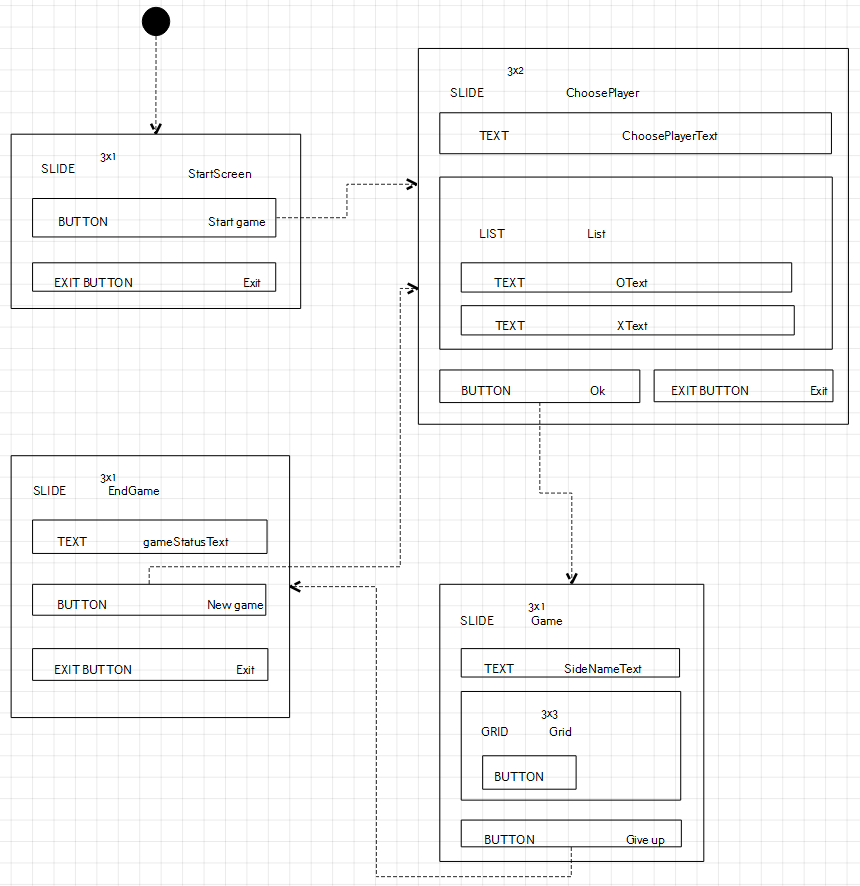
\includegraphics[width=0.9\textwidth]{part5/5.2/screenflow.png}
		\caption{Задание интерфейса приложения и переходов между экранами в QReal:Ubiq.}
		\label{image:screenflow}
	\end{center}
\end{figure}

Результатом реализации модельного примера (в качестве которого была выбрана игра "`Крестики-нолики"') 
стало то, что диаграммы переходов между формами оказались полезны сами по себе, поскольку 
хорошо визуализируют переходы, которые могут быть неочевидны в коде. Кроме того, по 
ним просто сгенерировать скелет приложения, а если сложная логика не требуется (например, 
приложение-визитка), то и приложение целиком. Однако задание сложной логики без кода 
на целевом языке привело к ещё более громоздким диаграммам, которые хоть и проще для 
понимания, чем диаграммы из прототипа, полученного на первом этапе работы, но всё 
же менее удобны, чем ручное кодирование.

\subsection{Результаты проекта QReal:Ubiq}
Первый этап проекта разрабатывался для мастер-класса в рамках конференции FRUCT 2011
%TODO: сноска
, где был успешно продемонстрирован, а на самой конференции был сделан доклад 
%TODO: ссылка
. На мастер-классе демонстрировалась разработка приложения для отображения данных 
с веб-камеры, аудитории был показан процесс создания и генерации логики клиентской 
части. Технология показалась весьма привлекательной авторам Ubiq Mobile, поэтому работа 
над ней была продолжена и после выступления.

С точки зрения исследования визуальных языков результаты проекта оказались менее однозначными: 
конечного ответа на вопрос "`возможно ли эффективно использовать визуальные языки 
вместо текстовых при решении достаточно общих задач"' получено не было. С одной стороны, 
визуальная технология дала очевидный выигрыш в том, что уменьшила объём необходимых 
для программирования знаний, с другой стороны, для некоторых задач, возникающих при 
разработке мобильного приложения, использование текстовых языков пока эффективнее. 

Работа над этим проектом поставила новые вопросы, требующие исследования. 
\begin{enumerate}
	\item Полноценная реализация редактора пользовательского интерфейса с визуализацией 
		переходов между формами (или экранами) средствами DSM-платформы. Для этого различные 
		элементы пользовательского интерфейса, такие как поля ввода, кнопки, выпадающие 
		списки и т.д. должны быть полноправными частями формы элемента языка.
	\item Поддержка работы с семействами визуальных языков, каждый из которых может 
		уточнять более общий язык под конкретную задачу. Таким образом может быть реализована 
		схема с настраиваемыми элементами из раздела~\ref{chapter:advancedQRealUbiq} --- 
		создать общий язык разработки мобильных приложений, от него породить язык задания 
		игр с полем, от него --- язык, содержащий специфические блоки для игры "`Морской бой"'. 
		Это не снимает всех проблем, перечисленных в разделе~\ref{chapter:advancedQRealUbiq} 
		касательно этой схемы, но представляется логичным развитием идей DSM-подхода.
\end{enumerate}
\section{Среда разработки аппаратуры QReal:HaSCoL}
Технология QReal:HaSCoL была исторически первой технологией, разработанной автором 
на платформе QReal, и именно опыт её разработки во многом определил направления дальнейших 
исследований и, в итоге, полученные в данной диссертации результаты. В частности, 
в ходе этой работы возникла потребность в визуальном метаредакторе. Данная технология 
не использует многих описанных в этой работе возможностей платформы QReal, поскольку 
на момент работы над ней эти возможности ещё не были реализованы, кроме того, сведения, 
приведённые в обзоре аналогичных подходов, могли устареть. Это не представляется критичным 
недостатком, поскольку основная цель дальнейшего изложения --- продемонстрировать 
пример разработки предметно-ориентированного визуального языка, причём для данной 
работы более важны методологические аспекты, чем специфика предметной области или особенности реализации конкретной DSM-платформы. 
% TODO: Убрать?
В этом плане предлагаемый пример интересен тем, что язык создавался и был строго формализован как расширение метамодели 
языка UML 2.0, поэтому данный опыт может быть использован для сравнения с более "`легковесными"' 
подходами, применявшимися в примерах из разделов~\ref{chapter:qRealRobots} и~\ref{chapter:qRealUbiq}.

\subsection{Постановка задачи}
Различные встроенные устройства играют большую роль в нашей жизни, однако задача их 
разработки всё ещё остаётся сложной и трудоёмкой. В 80-х годах двадцатого века появились языки Verilog и VHDL
%TODO: Сноски
, которые и по сей день остаются фактическим стандартом в деле разработки аппаратного 
обеспечения. Эти языки позволяют описать устройство аналогично коду обычной программы, 
их синтаксис похож на синтаксис традиционных языков программирования. Они позволяют 
синтезировать описание разрабатываемого аппаратного обеспечения, пригодное для производства, 
или произвести эмуляцию.

Тем не менее, данные языки заставляют описывать систему в низкоуровневых терминах, 
поэтому актуальна задача разработки новых технологий с более высоким уровнем абстракции. 
Визуальные методы разработки в данной предметной области даже более применимы, чем 
в области разработки ПО, поскольку аппаратное обеспечение традиционно описывалось 
различными чертежами и схемами. Однако же, в силу высокой (и постоянно растущей) сложности 
аппаратного обеспечения, средство визуального моделирования не может быть просто редактором 
электронных схем, а должно само поддерживать высокоуровневые концепции. Ещё одним 
важным требованием, накладываемым на такое средство, является исполнимость модели. 
Средство должно иметь возможность синтезировать описание устройства в виде, пригодном 
для использования промышленным оборудованием при производстве, и генерировать эмулятор 
устройства, позволяющий вести отладку, тестирование и оценку производительности, не 
прибегая к созданию дорогостоящего прототипа. Все эти сложности затрудняют разработку 
новых визуальных технологий.

На кафедре системного программирования математико-механического факультета СПбГУ разрабатывается 
текстовый язык разработки аппаратных систем HaSCoL (Hardware-Software Codesign Language)
% TODO: [ссылки], http://oops.math.spbu.ru/projects/coolkit
гораздо более высокого уровня, чем VHDL или Verilog. Перед автором данной диссертации 
была поставлена задача разработать визуальную технологию, которая бы использовала 
язык HaSCoL как целевой язык для генерации и позволяла бы проектировать аппаратуру 
в высокоуровневых терминах этого языка. Это дало бы возможность использовать инструментальные 
средства HaSCoL для создания как спецификации устройства для конфигурации FPGA
% TODO: Сноска
или производства, так и для генерации программного эмулятора. С другой стороны, визуальная 
технология должна была повысить удобство программирования на языке HaSCoL, а поскольку 
этот язык новый, это могло бы позитивно сказаться на эффективности его внедрения. 
Кроме того, использование высокоуровневого языка в качестве целевого для генерации 
свело бы к минимуму затраты на анализ предметной области при разработке DSM-решения, 
поскольку большая часть этой работы уже была выполнена при разработке текстового языка.

Язык HaSCoL описывает систему  в терминах исполняемых параллельно обработчиков сигналов.
Обработчики объединены в процессы --- сущности, инкапсулирующие в себе ресурсы (данные), 
обработчики сигналов и другие процессы, и имеющие входы и выходы. Обработчик представляет 
из себя последовательность однотактовых шагов, выполняющихся, если некоторые условия 
(получение сообщения, состояние ресурсов процесса) истинны. Обработчики могут начинать 
своё исполнение на каждом такте, на котором выполнены условия его старта, вне зависимости 
от того, выполняются они уже или нет. Пример описания процесса
%TODO (из работы [ссылка])
:

\vspace{5mm}
\begin{minipage}{\linewidth}
\begin{verbatim}
process DynamicArbiter =
begin
  in one(uint(2), uint(8));
  in two(uint(2), uint(8));
  out res(uint(8));
  group {
    -- что делать, если пришли оба сигнала:
    -- условия на принимаемые сигналы определяют готовность
    -- принятия данных из каждого входа в отдельности
    one(prio1, data1) and prio1 >= prio2,
    two(prio2, data2) and prio1 < prio2
    {
      send res (if prio1 >= prio2 then data1 else data2 fi)
    }
   -- если пришел только один сигнал --- случай попроще
   -- подчеркивание вместо имени параметра означает, что
   -- нас данный параметр не интересует и пользоваться им
   -- мы не будем
    one(_, ddata) {send res (ddata)}
    two(_, ddata) {send res (ddata)}
  }
end
\end{verbatim}
\end{minipage}
\vspace{5mm}

Процесс имеет два входа (one, two) с двумя параметрами и выход res, возвращающий значение 
типа uint(8). Конструкцией group три обработчика объединены в группу, перед фигурными 
скобками записано условие, при истинности которого обработчик начнёт работу, внутри 
фигурных скобок --- тело обработчика. В условиях могут участвовать проверки наличия 
данных на входах, логические выражения с участием входных данных и локальных данных 
процесса. Конструкция send в теле обработчика --- посылка сигнала на указанный выход. 
Входы и выходы могут также иметь несколько портов, каждый порт может быть связан с 
очередью сообщений. Например,

\begin{verbatim}
in InputData (int(16))[A[1], B];
\end{verbatim}
определяет вход с одним параметром и двумя портами, при этом размер очереди порта 
A --- 1, размер очереди порта B --- 0.

Для поддержки структурной декомпозиции процессов в язык был введён структурный уровень. 
Структурные конструкции позволяют отображать входы объемлющего процесса на порты входов 
вложенного, и выходы вложенного процесса на выходы объемлющего или входы вложенного, 
позволяя таким образом структурно декомпозировать процессы на наборы взаимодействующих 
вложенных подпроцессов.

Каждый процесс имеет свой тип, задаваемый явно или неявно. Тип процесса --- перечень 
его входов и выходов с указанием типов их аргументов. Над типами процессов определено 
отношение структурного сабтайпинга --- неформально говоря, процесс A имеет тип, являющийся 
подтипом типа процесса B, если A можно везде использовать вместо B. Тип процесса по 
умолчанию получается из спецификации процесса, тип можно указать и явно, это используется, 
например, для описания свойств параметров функторов.

Функтор --- это процесс, параметризованный другим процессом. Например,

\vspace{5mm}
\begin{minipage}{\linewidth}
\begin{verbatim}
process Wrapper (P: Proc) =
begin
  process X = P;
  process Y = P;
  ...
end
\end{verbatim}
\end{minipage}
\vspace{5mm}

Процесс Wrapper параметризован процессом P типа Proc. Применение функтора выглядит так:
\begin{verbatim}
process W = Wrapper(aProc);
\end{verbatim}

\subsection{Существующие средства визуального описания аппаратных систем}
Самый известный из существующих визуальных языков, UML 2, создавался с учётом необходимости 
описывать аппаратные средства. В версиях UML 1.x специальных средств для описания 
аппаратных систем не было, поэтому приходилось создавать профили UML, например, UML-RT.
% TODO: ссылка 
В UML 2 этот пробел был заполнен, в язык было введено понятие "`структурированный классификатор"', 
который может содержать внутри себя набор частей, соединённых между собой соединителями. 
Взаимодействие структурированных классификаторов с внешним миром и внутренними частями 
происходит исключительно через порты. Порт --- это точка взаимодействия со строго 
определённым интерфейсом. Один структурированный классификатор может иметь несколько 
портов, а также имеет возможность определить, на какой из портов пришёл запрос. Запросы, 
приходящие на порты, могут быть обработаны непосредственно объектом-хозяином порта 
или переданы на порт какой-либо его части. Каждый порт имеет набор предоставляемых 
им интерфейсов и набор интерфейсов, требуемых от внешней среды. Пример нотации представлен 
на рисунке~\ref{image:umlStructuredClassifier}.

\begin{figure} [ht]
	\begin{center}
		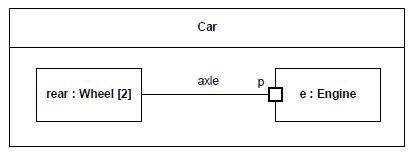
\includegraphics[width=0.6\textwidth]{part5/5.3/umlStructuredClassifier.png}
		\caption{Структурированный классификатор UML 2.}
		\label{image:umlStructuredClassifier}
	\end{center}
\end{figure}

Для задания внутреннего поведения элементов системы в UML 2 обычно используется диаграмма 
конечных автоматов. Каждый структурированный классификатор может иметь связанный с 
ним конечный автомат, который описывает реакцию на события, приходящие на его порты.

Помимо "`чистого"' UML 2 используются и специальные профили UML, предназначенные для 
использования с текстовыми языками (подход, весьма близкий к предлагаемому). Пример 
такого профиля --- 
% TODO: представленный в работе [ссылка] 
профиль UML для языка SystemC. SystemC
% TODO [ссылка] 
--- язык проектирования уровня системы, основанный на C++ и поддерживаемый группой крупных компаний. 
% TODO: Каких?
Система в SystemC состоит из модулей, каждый модуль может содержать переменные, порты 
для взаимодействия с окружением и процессы, реализующие функциональность модуля. Процессы
исполняются параллельно и могут реагировать на события. Связь между модулями осуществляется 
с помощью портов, которые предоставляют модулям доступ к каналам. Каналы бывают примитивными 
и иерархическими: иерархический канал --- тоже модуль, имеет свои процессы и может иметь 
доступ к другим каналам.

Профиль UML для SystemC логически разделён на 3 части.
\begin{enumerate}
	\item Структуры и коммуникации --- определяет стереотипы для базовых строительных 
		блоков SystemC. Эти стереотипы представляют модули, порты, интерфейсы и каналы, 
		и используются на различных диаграммах UML, например, на диаграммах классов и 
		диаграммах композитных структур.
	\item Поведение и синхронизация --- определяет стереотипы для спецификации поведения 
		процессов SystemC. Эти стереотипы используются в диаграммах состояний UML.
	\item Типы данных --- представляет типы данных SystemC.
\end{enumerate}

Пример нотации профиля UML для SystemC представлен на рисунке~\ref{image:systemCExample}.

\begin{figure} [ht]
	\begin{center}
		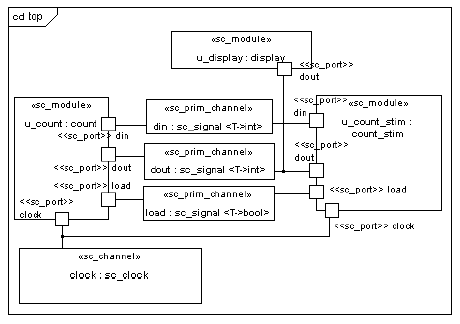
\includegraphics[width=0.8\textwidth]{part5/5.3/systemCExample.png}
		\caption{Пример нотации профиля для SystemC.}
		\label{image:systemCExample}
	\end{center}
\end{figure}

Как видно из обзора, идея визуального моделирования аппаратного обеспечения не нова, 
при этом наибольшее внимание уделяется языку UML (по-видимому, как наиболее распространённому 
визуальному языку). При этом, существующие языки пытаются целиком специфицировать 
систему графическими средствами, что зачастую приводит к весьма громоздким диаграммам.

\subsection{Предлагаемый набор визуальных языков}
Основные принципы, в соответствии с которыми разрабатывалась нотация, таковы.
\begin{enumerate}
	\item Модель должна быть исполняемой, то есть позволять синтезировать код на языке 
		системы CoolKit без необходимости ручной корректировки результатов. Пригодная 
		для промышленного использования технология должна позволять программисту получать 
		готовую низкоуровневую спецификацию системы или эмулятор, действуя в одной среде 
		разработки и, желательно, с одним представлением системы.
	\item Графическими примитивами должны быть представлены только те элементы программы, 
		которые наиболее выгодно представлять графически. Остальная необходимая для синтеза 
		информация должна быть представлена на визуальной модели в текстовой форме. Такой 
		подход позволяет сохранять диаграммы достаточно компактными, но при этом, как 
		обсуждалось в разделе~\ref{chapter:qRealUbiq}, делает программы существенно более 
		сложными для понимания.
	\item Нотация разрабатывалась для использования внутри среды разработки, поэтому 
		некоторые её элементы могут быть неудобны для представления на бумаге.
\end{enumerate}

Для визуализации языка CoolKit плохо подходит непосредственно UML и даже профиль для 
UML --- целевой язык не является строго говоря объектно-ориентированным, к тому же 
обладает рядом особенностей, которые плохо или неудобно выражаются в терминах UML. 
Предлагаемый графический язык, хотя и не является профилем UML, сформулирован с активным 
использованием метамодели UML. Для формализации языка используется метамоделирование 
на метаязыке MOF --- синтаксис графических конструкций языка описан с помощью диаграмм UML. 
Метамодель языка построена на метамодели ядра и некоторых диаграмм UML, таким образом, 
язык лишь незначительно отличается от UML и его синтаксис и семантика интуитивно понятны 
специалистам, занимающимся визуальным моделированием. Кроме того, переиспользование 
метамодели UML позволило сэкономить массу усилий при формализации языка. Одним из 
полученных результатов стало понимание того, что формализация предметно-ориентированных 
языков программирования может быть существенно упрощена благодаря переиспользованию 
некоей стандартной метамодели, например UML.

Для спецификации системы в нашем языке используется два вида диаграмм --- диаграмма 
типов процессов и диаграмма отображения портов. Заметим, что мы избежали необходимости 
использовать диаграммы автоматов для описания поведения системы --- эту роль выполняют 
текстовые блоки на целевом языке. Диаграмма типов процессов базируется на диаграмме 
классов UML, а диаграмма отображения портов --- на диаграмме композитных структур.

\subsubsection{Диаграмма типов процессов}
Диаграмма типов процессов используется для задания основных структурных свойств и 
отношений процессов, составляющих пакет или приложение. На диаграмме изображаются сами 
процессы, их входы и выходы, отношения вложенности, отношения генерализации, и функторы. 
Заметим, что на этой диаграмме не рисуются обработчики событий, и могут не рисоваться 
ресурсы процесса (список ресурсов процесса может быть неполным, из того, что ресурс 
не изображён на диаграмме, нельзя делать вывод, что он не описан в процессе). Некоторые 
вложенные процессы тоже могут быть опущены на этой диаграмме, если это не повлияет 
на корректность модели. Часть метамодели диаграммы представлена на рисунке~\ref{image:processTypesMetamodel}.

\begin{figure} [ht]
	\begin{center}
		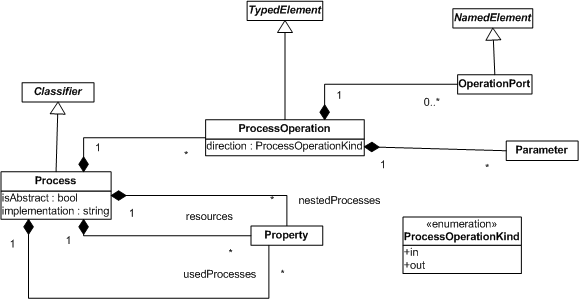
\includegraphics[width=0.9\textwidth]{part5/5.3/processTypesMetamodel.png}
		\caption{Метамодель диаграммы типов процессов.}
		\label{image:processTypesMetamodel}
	\end{center}
\end{figure}

Пример изображения вложенных процессов представлен на рисунке~\ref{image:processTypesNotation}. 
Как видно из примера, нотация перечисляет ресурсы, входы и выходы процессов в таком 
виде, в каком они были в языке системы CoolKit. По-настоящему графически здесь изображаются 
только отношения использования одного процесса внутри другого или вложенности процессов 
(т.е. когда один процесс описан непосредственно внутри другого). Заметим, что вложенный 
процесс может не иметь имени --- тогда оно просто не отображается на диаграмме. Поскольку 
вложенные или используемые процессы являются деталями реализации объемлющего процесса, 
они могут не рисоваться на диаграмме. 

\begin{figure} [ht]
	\begin{center}
		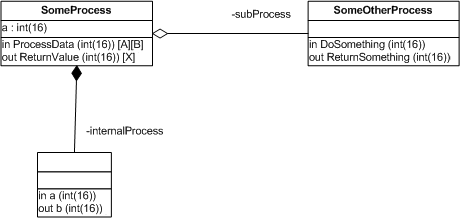
\includegraphics[width=0.7\textwidth]{part5/5.3/processTypesNotation.png}
		\caption{Нотация процессов.}
		\label{image:processTypesNotation}
	\end{center}
\end{figure}

Существенную выгоду от использования этого типа диаграммы можно получить при использовании 
в программе функторов. Пример нотации объявления функторов приведён на рисунке~\ref{image:functorsNotation}. 

\begin{figure} [ht]
	\begin{center}
		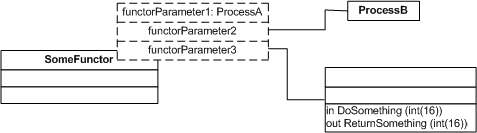
\includegraphics[width=0.7\textwidth]{part5/5.3/functorsNotation.png}
		\caption{Нотация функторов.}
		\label{image:functorsNotation}
	\end{center}
\end{figure}

В частности, из-за особенности нотации, которую можно видеть на примере, было принято 
решение не использовать диаграммы классов UML. Нотация отражает возможность языка 
системы CoolKit описывать тип процесса --- формальный параметр функтора прямо в месте 
описания формального параметра. Вынесение типов параметров в отдельные графические 
сущности позволяет сделать отношения между процессами --- формальными или фактическими 
параметрами функторов гораздо более наглядными. Применение функтора изображается так, 
как показано на рисунке~\ref{image:functorApplication}.

\begin{figure} [ht]
	\begin{center}
		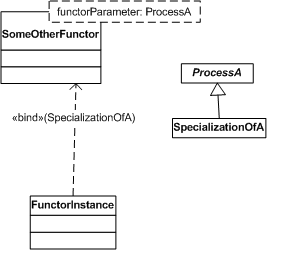
\includegraphics[width=0.5\textwidth]{part5/5.3/functorApplication.png}
		\caption{Применение функтора.}
		\label{image:functorApplication}
	\end{center}
\end{figure}

Для того, чтобы проиллюстрировать применение диаграммы типов процессов, рассмотрим 
содержательный пример --- задачу об арбитре динамических приоритетов 4 в 1
%TODO: из [ссылка] 
. Задача формулируется следующим образом: на один из четырёх входов поступают данные, 
первый параметр пришедших данных --- приоритет. Если в одном такте данные поступили 
на несколько входов, на выход выдаются данные с наибольшим приоритетом, остальные 
входы объявляются неготовыми. Если приходит только одно сообщение, оно отправляется 
на выход.

Следуя оригинальному решению поступим следующим образом --- сначала напишем арбитр 
динамических приоритетов 2 в 1 (с двумя входами и одним выходом), затем создадим арбитр-функтор 
4 в 1, использующий 3 арбитра 2 в 1, который и решит задачу (см. рисунок~\ref{image:arbiter4To1ProcessTypes}). 

\begin{figure} [ht]
	\begin{center}
		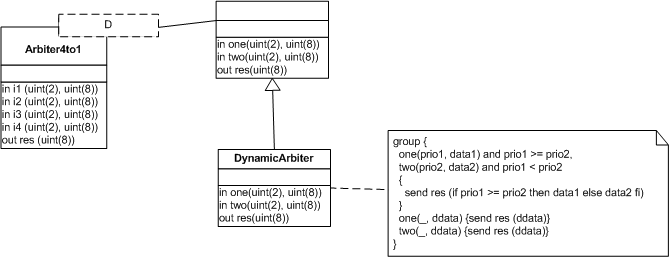
\includegraphics[width=\textwidth]{part5/5.3/arbiter4To1ProcessTypes.png}
		\caption{Диаграмма типов процессов для задачи "`Арбитр 4 в 1"'.}
		\label{image:arbiter4To1ProcessTypes}
	\end{center}
\end{figure}

В комментарии --- код процесса DynamicArbiter на языке системы CoolKit, описывающий 
реализацию арбитра 2 к 1. Код из комментария при синтезе добавляется к сгенерированному 
описанию процесса, таким образом мы получаем полностью специфицированный арбитр 2 к 1, 
который может быть использован как фактический параметр функтора Arbiter4to1 (на это 
указывает отношение генерализации, связывающее DynamicArbiter и безымянный тип процесса --- 
формальный параметр функтора). Про процесс Arbiter4to1 мы указали пока только то, 
что он является функтором (готов использовать любой процесс, поддерживающий интерфейс 
арбитра 2 к 1, который мы определили с помощью безымянного типа процесса), и указали, 
что у него есть 4 входа и один выход --- то есть просто "нарисовали" условие задачи.

\subsubsection{Диаграмма отображения портов}
Диаграмма отображения портов рисуется для отдельного процесса и используется для отображения 
связей между входными и выходными портами вложенных процессов того процесса, для которого 
рисовалась диаграмма. Таким образом, эта диаграмма фактически является графической 
нотацией для структурного уровня языка системы CoolKit. Синтаксис с незначительными 
изменениями совпадает с синтаксисом диаграммы составных структур UML. На диаграмме 
изображаются процессы и их порты (все порты входов и выходов), связи между портами, 
внутри процессов могут находиться вложенные процессы. Важно различие между процессом 
верхнего уровня --- процессом, относительно которого рисуется диаграмма, и вложенными 
процессами. Вложенные процессы на самом деле являются экземплярами процессов, имеют 
имя и тип. Процесс верхнего уровня имеет только тип. Пример нотации изображён на рисунке~\ref{image:portMappingsExample}. 
Вернёмся к нашему примеру с арбитром 4 к 1. Диаграмма отображения портов для этого примера 
выглядит так, как показано на рисунке~\ref{image:arbiter4To1PortMappings}.

\begin{figure} [ht]
	\begin{center}
		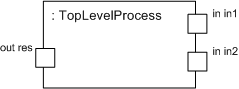
\includegraphics[width=0.4\textwidth]{part5/5.3/portMappingsExample.png}
		\caption{Процесс на диаграмме отображения портов.}
		\label{image:portMappingsExample}
	\end{center}
\end{figure}

\begin{figure} [ht]
	\begin{center}
		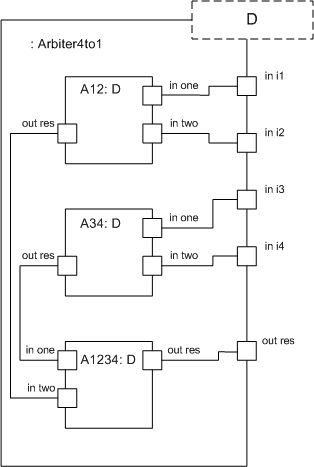
\includegraphics[width=0.5\textwidth]{part5/5.3/arbiter4To1PortMappings.png}
		\caption{Диаграмма отображения портов для задачи "`Арбитр 4 в 1"'.}
		\label{image:arbiter4To1PortMappings}
	\end{center}
\end{figure}

Здесь мы видим процесс верхнего уровня Arbiter4to1 --- без имени, но с типом и с формальным 
параметром функтора. Arbiter4to1 имеет 4 входных порта и 1 выходной, их типы здесь 
уже можно не указывать, они были на диаграмме типов процессов, которую мы нарисовали 
ранее. Процесс имеет три вложенных процесса A12, A34 и A1234 типа D, который, как 
следует из диаграммы типов процессов, описывает процессы, имеющие два входа и один 
выход. Если мы считаем, что в качестве параметра функтора передаётся арбитр 2 к 1, 
изображённое на рисунке соединение портов решает задачу.

\subsubsection{Генерация}
Генерация в язык системы CoolKit проходит довольно очевидным образом, поскольку графический 
и текстовый языки имеют одинаковую модель представления аппаратного устройства. Скелеты 
описаний процессов генерируются по диаграмме типов процессов, потом они дополняются 
вложенными процессами и конструкциями, описывающими связь портов по диаграмме отображения 
портов, потом они дополняются реализацией, которая так или иначе представлена в текстовом 
виде на диаграмме --- в виде комментария или в виде неотображаемого атрибута процесса. 
В результате получается полная программа на языке системы CoolKit, готовая к дальнейшей 
трансляции в VHDL и далее --- в эмулятор или спецификацию устройства.

При генерации считается, что одноимённые однотипные сущности в одном пространстве 
имён представляют собой одну сущность. То есть, например, если на одной диаграмме 
описан процесс с одним входом, а на другой диаграмме описан процесс с тем же именем 
и другим входом, будет сгенерирован один процесс с двумя входами. Такой подход позволяет 
изображать на каждой диаграмме только существенные для неё части системы, хотя и может 
привести к некоторой сложности для понимания набора диаграмм в целом. Предполагается, 
что у средства визуального моделирования существует возможность удобным способом предоставить 
пользователю информацию о невидимых на диаграмме элементах. Есть некоторые тонкости 
с тем, что разные формально сущности на разных диаграммах представляют собой одну 
логическую сущность, например, процесс на диаграмме типов процессов и процесс на диаграмме 
отображения портов. Такие сущности всё же должны считаться генерацией однотипными и 
объединяться в одну сущность. Например, двух ранее приведённых диаграмм, описывающих 
реализацию арбитра 4 к 1, достаточно, чтобы сгенерировать такой код на языке системы CoolKit:

\vspace{5mm}
\begin{minipage}{\linewidth}
\begin{verbatim}
process DynamicArbiter =
begin
  in one(uint(2), uint(8));
  in two(uint(2), uint(8));
  out res(uint(8));
  group {
    one(prio1, data1) and prio1 >= prio2,
    two(prio2, data2) and prio1 < prio2
    {
      send res (if prio1 >= prio2 then data1 else data2 fi)
    }
    one(_, ddata) {send res (ddata)}
    two(_, ddata) {send res (ddata)}
  }
end

process Arbiter4to1 (D : begin
  in one(uint(2), uint(8));
  in two(uint(2), uint(8));
  out res(uint(8));
  end
) =
begin
  in i1 (uint(2), uint(8));
  in i2 (uint(2), uint(8));
  in i3 (uint(2), uint(8));
  in i4 (uint(2), uint(8));
  out res (uint(8));
  process A12 = D with one = i1, two = i2, res = A1234.one;
  process A34 = D with one = i3, two = i4, res = A1234.two;
  process A1234 = D with res = res;
end
\end{verbatim}
\end{minipage}
\vspace{5mm}

Для того, чтобы получить исполнимый код, нужно создать экземпляр процесса Arbiter4to1, 
использующий в качестве параметра процесс DynamicArbiter. Для этого достаточно нарисовать 
диаграмму, изображённую на рисунке~\ref{image:arbiter4To1FunctorApplication}.

\begin{figure} [ht]
	\begin{center}
		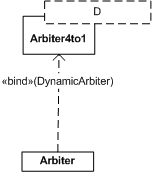
\includegraphics[width=0.2\textwidth]{part5/5.3/arbiter4To1FunctorApplication.png}
		\caption{Применение функтора "`Арбитр 4 к 1"'.}
		\label{image:arbiter4To1FunctorApplication}
	\end{center}
\end{figure}

Эта диаграмма породит код 

\begin{verbatim}
process Arbiter = Arbiter4to1(DynamicArbiter);
\end{verbatim}

Этот код вместе с приведённым ранее кодом может быть синтезирован и исполнен на эмуляторе.

\subsection{Результаты проекта QReal:HaSCoL}
В результате работы над технологией QReal:Hascol было создано два языка, с помощью 
которых описывалась структурная часть системы. Технология не была доведена до промышленного 
использования, полученные результаты нигде не публиковались, связано это с недостаточной 
зрелостью базовой технологии QReal на момент работы над QReal:HaSCoL. Однако проблемы, 
возникшие при разработке, во многом послужили мотивацией для реализации тех возможностей 
метатехнологии QReal, которые представляются в данной работе. Кроме того, визуальный язык 
QReal:HaSCoL далее использовался как пример для апробации различных новых возможностей 
QReal, например, "`метамоделирования на лету"'.
%TODO: [ссылка на диплом Жени][ссылка на курсовую Птахиной].

С точки зрения введённой в данной работе классификации созданные языки являются статическими 
текстовографическими языками. В данном случае использование текстовой нотации не так 
осложняет понимание диаграмм, как в случае QReal:Ubiq (раздел~\ref{chapter:qRealUbiq}), 
поскольку текстовая и графическая части не взаимозаменяемы: структурная часть системы 
целиком описывается графически, поведенческая --- целиком текстово. Были предприняты 
попытки использовать диаграммы активностей языка UML 2.0 для задания и поведенческой 
части в графическом виде, но в результате получались громоздкие и трудночитаемые диаграммы, 
поэтому было принято решение поведенческую часть задавать в текстовом виде.

В отличие от всех последующих языков на базе платформы QReal, языки QReal:HaSCoL создавались 
на базе метамодели UML 2.0. Это было сделано для того, чтобы строго формализовать 
язык и сделать возможной его реализацию не только на базе QReal (впрочем, таких попыток 
не предпринималось), а также опробовать на реальном примере такой подход к разработке 
синтаксиса языка. Результаты показали, что переиспользование метамодели UML действительно 
позволяет сэкономить много усилий (потребовалось ввести всего две-три новые сущности 
на каждый язык из семейства), однако от разработчика требуется хорошо ориентироваться
в метамодели UML, что само по себе весьма непросто. Стандарт UML достаточно объёмен, 
а метамодель весьма запутанна (особую сложность для читаемости метамодели представляет 
активное использование операций объединения пакетов PackageMerge и использование сущностей 
с одинаковыми именами в разных пакетов). Как кажется, затраты на изучение метамодели 
UML превышают выгоду, получаемую от переиспользования этой метамодели, так что разрабатывать 
новый предметно-ориентированный язык "`с нуля"' с использованием метаязыка выбранной 
DSM-платформы более оправданно, чем перед созданием языка специально изучать метамодель 
UML. Наличие эффективных инструментальных средств, помогающих разобраться в больших 
метамоделях наподобие UML и автоматизировать переиспользование фрагментов метамодели, 
как кажется, смогло бы изменить ситуацию, однако на данный момент такие средства не 
распространены, и создание таких средств представляется интересным направлением дальнейших 
исследований.
